\let\negmedspace\undefined
\let\negthickspace\undefined
\documentclass[journal]{IEEEtran}
\usepackage[a5paper, margin=10mm, onecolumn]{geometry}
%\usepackage{lmodern} % Ensure lmodern is loaded for pdflatex
\usepackage{tfrupee} % Include tfrupee package

\setlength{\headheight}{1cm} % Set the height of the header box
\setlength{\headsep}{0mm}  % Set the distance between the header box and the top of the text

\usepackage{gvv-book}
\usepackage{gvv}
\usepackage{cite}
\usepackage{amsmath,amssymb,amsfonts,amsthm}
\usepackage{algorithmic}
\usepackage{graphicx}
\usepackage{textcomp}
\usepackage{xcolor}
\usepackage{txfonts}
\usepackage{listings}
\usepackage{enumitem}
\usepackage{mathtools}
\usepackage{gensymb}
\usepackage{comment}
\usepackage[breaklinks=true]{hyperref}
\usepackage{tkz-euclide} 
\usepackage{listings}
% \usepackage{gvv}                                        
\def\inputGnumericTable{}                                 
\usepackage[latin1]{inputenc}                                
\usepackage{color}                                            
\usepackage{array}                                            
\usepackage{longtable}                                       
\usepackage{calc}                                             
\usepackage{multirow}                                         
\usepackage{hhline}                                           
\usepackage{ifthen}                                           
\usepackage{lscape}
\begin{document}

\bibliographystyle{IEEEtran}
\vspace{3cm}

\title{7.2.29}
\author{EE24BTECH11021 - Eshan Ray}

% \maketitle
% \newpage
% \bigskip
{\let\newpage\relax\maketitle}

\renewcommand{\thefigure}{\theenumi}
\renewcommand{\thetable}{\theenumi}
\setlength{\intextsep}{10pt} % Space between text and floats
\textbf{Question: }\\
A circle drawn with origin as the centre passes through $\brak{\frac{13}{2},0}$. The point which does not lie in the interior of the circle is
\begin{enumerate}
    \item $\brak{\frac{-3}{4},1}$
    \item $\brak{2,\frac{7}{3}}$
    \item $\brak{5,\frac{-1}{2}}$
    \item $\brak{-6,\frac{-5}{2}}$
\end{enumerate}
\solution {
\begin{table}[h!]    
  \centering
  \begin{tabular}[12pt]{ |c| c|}
    \hline
        \textbf{Variable}  & \textbf{Description} \\
    \hline
        $\vec{B}$$\brak{-4,0}$ &  coordinates of first point  \\
    \hline 
        $\vec{C}$$\brak{10,0}$ & coordinates of second point \\
    \hline
        $\vec{A}$& Equidistant point of $\vec{B}$ and $\vec{C}$ on $X$ axis \\  
    \hline
         
\end{tabular}

  \caption{Input parameters}
  \label{tab1.1.9.2}
\end{table}
\\
    As $A$ lies on circle,
    \begin{align}
        \norm{A}^2 + 2u^\top A +f&=0\\
        \implies f&= -\brak{\brak{\frac{13}{2}}^2} - 2\myvec{0 & 0}\myvec{\frac{13}{2}\\ 0}\\
        \implies f&= -\frac{169}{4}
        \end{align}
        $\therefore$ The equation of the circle is $\norm{x}^2=\frac{169}{4}$.\\ \\
        A point is inside the circle if $\norm{P-O}^2<r^2$\\
            $r^2=\frac{169}{4}=42.25$\\ \\
        For $B\brak{\frac{-3}{4},1}$
        \begin{align}
            \norm{B-O}^2 &= \norm{\myvec{\frac{-3}{4}\\1}-\myvec{0\\0}}^2\\
            \implies \norm{B-O}^2&=\norm{\myvec{\frac{-3}{4}\\ 1}}^2\\
            \implies \norm{B-O}^2&= \brak{\frac{-3}{4}}^2 +1^2\\
            \implies \norm{B-O}^2&= \frac{25}{16}<\frac{169}{4}\\
            \implies \norm{B-O}^2<r^2
        \end{align}
        So, $B\brak{\frac{-3}{4},1}$ lies inside the circle.\\ \\
         For $C\brak{2,\frac{7}{3}}$
        \begin{align}
             \norm{C-O}^2 &= \norm{\myvec{2\\ \frac{7}{3}}-\myvec{0\\0}}^2\\
            \implies \norm{C-O}^2&=\norm{\myvec{2\\ \frac{7}{3}}}^2\\
            \implies \norm{C-O}^2&= 2^2 +\brak{\frac{7}{3}}^2\\
            \implies \norm{C-O}^2&= \frac{85}{9}<\frac{169}{4}\\
            \implies \norm{C-O}^2<r^2
        \end{align}
        So, $C\brak{2,\frac{7}{3}}$ lies inside the circle.\\ \\
        For $D\brak{5,\frac{-1}{2}}$
        \begin{align}
             \norm{D-O}^2 &= \norm{\myvec{5\\ \frac{-1}{2}}-\myvec{0\\0}}^2\\
            \implies \norm{D-O}^2&=\norm{\myvec{5\\ \frac{-1}{2}}}^2\\
            \implies \norm{D-O}^2&= 5^2 +\brak{\frac{-1}{2}}^2\\
            \implies \norm{D-O}^2&= \frac{101}{4}<\frac{169}{4}\\
            \implies \norm{D-O}^2<r^2
        \end{align}
         So, $D\brak{5,\frac{-1}{2}}$ lies inside the circle.\\ \\
         For $E\brak{-6,\frac{-5}{2}}$
         \begin{align}
             \norm{E-O}^2 &= \norm{\myvec{-6\\ \frac{-5}{2}}-\myvec{0\\0}}^2\\
            \implies \norm{E-O}^2&=\norm{\myvec{-6\\ \frac{-5}{2}}}^2\\
            \implies \norm{E-O}^2&= \brak{-6}^2 +\brak{\frac{-5}{2}}^2\\
            \implies \norm{E-O}^2&= \frac{169}{4}=\frac{169}{4}\\
            \implies \norm{E-O}^2=r^2
         \end{align}
         So, only point $E\brak{-6,\frac{-5}{2}}$ lies on the circle.
         \begin{figure}[!ht]
    \centering
	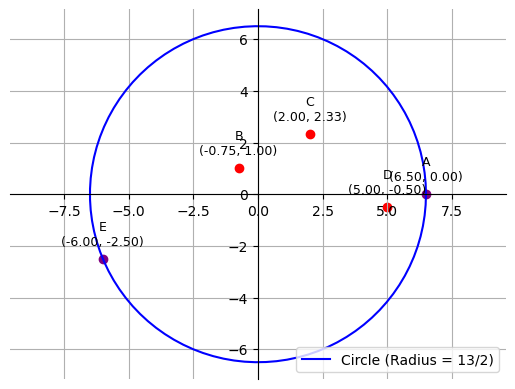
\includegraphics[width=1\textwidth]{plots/plot.png}
    \caption{Point E lies on the circle}
    \label{fig:plot}
\end{figure}  
}
\end{document}
